Traditionally, 
protein function was tightly associated with structure,
but this is only part of the picture.
Many different biophysical features determine protein function:
structure,
hydrophobicity,
backbone and sidechain dynamics,
early folding propensity,
aggregation propensity,
solvent exposure,
and many more.
And essentially all are encoded within the primary sequence.
Extracting them remains challenging, but many efforts are being made,
as extracting biophysical features and to understand their relation to sequence space would greatly improve our understanding in proteins (Fig. \ref{fig:sequence_feature_relation}).
It would also help advance the field of protein design.
It is considered by some to have potential similar the to industrial revolution by the many application in 
medicine,
genetic circuit design,
bottom up nano technology,
and much more.


~\begin{figure}[h!]
	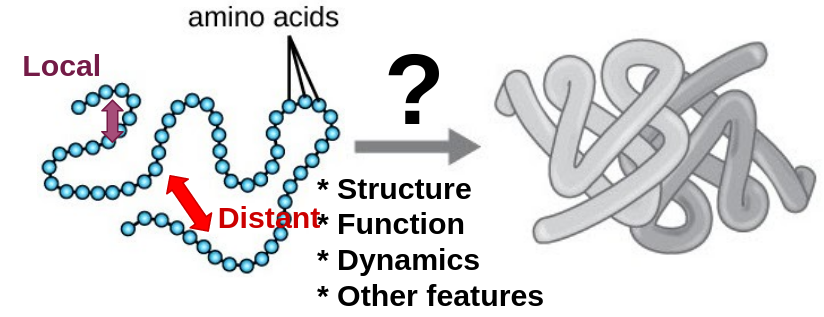
\includegraphics[width=\linewidth]{./literature_review/feature_prediction/biophysical_landscape/img/feature_prediction.png}
	\caption{\textbf{The protein sequence encodes its biophysical features.}
Local and distant interactions in protein sequence determine its biophysical properties,
but the mechanism are still a topic of active research.
}	
	\label{fig:sequence_feature_relation}
~\end{figure}

